% SIAM Article Template
\documentclass[review,hidelinks,onefignum,onetabnum]{siamart220329}

% Information that is shared between the article and the supplement
% (title and author information, macros, packages, etc.) goes into
% ex_shared.tex. If there is no supplement, this file can be included
% directly.

% SIAM Shared Information Template
% This is information that is shared between the main document and any
% supplement. If no supplement is required, then this information can
% be included directly in the main document.


% Packages and macros go here
\usepackage{lipsum}
\usepackage{amsfonts}
\usepackage{graphicx}
\usepackage{epstopdf}
\usepackage{algorithmic}
\usepackage{amsmath}
%\usepackage{natbib}
\ifpdf
  \DeclareGraphicsExtensions{.eps,.pdf,.png,.jpg}
\else
  \DeclareGraphicsExtensions{.eps}
\fi

% Add a serial/Oxford comma by default.
\newcommand{\creflastconjunction}{, and~}

% Used for creating new theorem and remark environments
\newsiamremark{remark}{Remark}
\newsiamremark{hypothesis}{Hypothesis}
\crefname{hypothesis}{Hypothesis}{Hypotheses}
\newsiamthm{claim}{Claim}

% Sets running headers as well as PDF title and authors
\headers{An Example Article}{D. Doe, P. T. Frank, and J. E. Smith}

% Title. If the supplement option is on, then "Supplementary Material"
% is automatically inserted before the title.
\title{Restarting the non-symmetric Lanczos algorithm via the implicitly shifted LR algorithm\thanks{Submitted to the editors DATE.
\funding{This work was funded by the Fog Research Institute under contract no.~FRI-454.}}}

% Authors: full names plus addresses.
\author{P. S. Negi\thanks{Imagination Corp., Chicago, IL 
  (\email{prabal.negi@su.se}, \url{http://www.imag.com/\string~ddoe/}).}
\and C. Arratia\thanks{Department of Applied Mathematics, Fictional University, Boise, ID 
  (\email{cristobal.arratia@su.se}).}
}

\usepackage{amsopn}
\DeclareMathOperator{\diag}{diag}


%%% Local Variables: 
%%% mode:latex
%%% TeX-master: "ex_article"
%%% End: 


% Optional PDF information
\ifpdf
\hypersetup{
  pdftitle={An Example Article},
  pdfauthor={D. Doe, P. T. Frank, and J. E. Smith}
}
\fi

\newcommand{\Citation}{(\textbf{Citation}) }

% The next statement enables references to information in the
% supplement. See the xr-hyperref package for details.

\externaldocument[][nocite]{ex_supplement}

% FundRef data to be entered by SIAM
%<funding-group specific-use="FundRef">
%<award-group>
%<funding-source>
%<named-content content-type="funder-name"> 
%</named-content> 
%<named-content content-type="funder-identifier"> 
%</named-content>
%</funding-source>
%<award-id> </award-id>
%</award-group>
%</funding-group>

\begin{document}

\maketitle

% REQUIRED
\begin{abstract}
The shifted QR iteration is used as a restart procedure for the Arnoldi method for the calculation of a few eigenvalues of a large matrix. We show that the underlying idea can be utilized in much the same manner via the shifted LR iteration to create a restart procedure for the non-symmetric Lanczos algorithm for eigenvalue calcuations. Additionally, we show that the (shifted) LR iteration can be performed implicitly in a manner similar to the Francis' algorithm, resulting in a bulge-chase type procedure which does not require the explicit construction of the full lower and upper triangular matrices. 
\end{abstract}

% REQUIRED
\begin{keywords}
LR algorithm, unsymmetric Lanczos, implicit restart
\end{keywords}

% REQUIRED
\begin{MSCcodes}
68Q25, 68R10, 68U05
\end{MSCcodes}

\section{Introduction}
The Arnoldi iteration \cite{arnoldi51} is a popular Krylov space method for calculating a few eigenvalues of a large matrix. The method relies on the generation of a sequence of Krylov vectors which determine the subspace within which approximations of the eigenvalue-eigenvector pairs are obtained. Depending on the accuracy and number of eigenpair approximations needed, the Krylov space size can become exceedingly large so that  the quality of the results may be limited by the available memory. Sorensen \cite{sorensen92} introduced an elegant procedure for restarting the Arnoldi factorization based on polynomial filters, which are applied through the implicitly shifted QR iterations on the reduced Hessenberg matrix obtained through the Arnoldi method. In particular, the use of exact shifts was shown to be successful in the convergence process of the eigenspace\cite{sorensen92} of the specified eigenvalues. The method has subsequently found widespread application through the ARPACK library \cite{arpack98}. The use of QR iterations ensures that the reduced matrix preserves its Hessenberg structure through the transforms that make up the restart process. If the underlying matrix is symmetric, the Arnoldi iteration reduces to the Lanczos algorithm and, the Hessenberg matrix reduces to a symmetric tridiagonal matrix. The QR iteration preserves the symmetric tridiagonal structure as well and, as pointed out by Sorensen \cite{sorensen92}, the implicit restart process applies equally well for the Lanczos method for symmetric matrices. 

One would like to extend this procedure to the case of the non-symmetric Lanczos method. However, the reduced matrix that one obtains is a non-symmetric tridiagonal matrix, with the tridiagonal structure being the result of the recurrence relations of the Lanczos algorithm \cite{saad82}. Since the QR iterations do not preserve the banded structure of non-symmetric matrices, a straightforward application of the restart procedure propounded by Sorensen will lead to a loss of this tridiagonal structure of the reduced matrix (the Hessenberg structure will still be preserved).  This loss of structure can be circumvented if one looks to the predecessor of the QR algorithm namely, the LR algorithm proposed by Rutihauser \cite{rutishauser58,rutishauser63,rutihauser91}, which has the attractive property of preserving the band structure of a matrix. This property was already pointed out by Rutihauser in \cite{rutishauser58} where the banded matrices were referred to as striped matrices. As we will show in the next section, shifted LR transforms is the appropriate generalization of the restart procedure to the case of non-symmetric Lanczos iteration. The process would necessarily require refining both the right as well as the left Krylov spaces simultaneously.

The rest of the paper is organized as follows. In the next section we start with the introduction of the non-symmetric Lanczos iteration and then develop the restart procedure. We also show that the LR algorithm can be implemented as a bulge-chase method, similar to the Francis' algorithm. In section 3 we apply the restart process to the Grcar matrix, and make some concluding remarks in section 4.

\section{Non-symmetric Lanczos}
Lanczos first introduced his algorithm in \cite{lanczos50} as a method for tridiagonalizing a matrix, but also realized that the method could be used iteratively to find eigenvalues. For an arbitry matrix $A$, the method generates a pair of Krylov subspaces $\{v_{1},\ldots,v_{j}\}$ and $\{w_{1},\ldots,w_{j}\}$, through repeated action of $A$ and $A^{H}$ respectively. We refer to these as the right and left Krylov spaces respectively and they satisfy the biorthogonality relation $w_{i}^{H}v_{j}=\delta_{ij}$. The two subspaces are generated through the following recurrence relations:
\begin{subequations}
\begin{eqnarray}
	\delta_{j+1}v_{j+1} = Av_{j} - \alpha_{j}v_{j} - \beta_{j}v_{j-1} \label{eqn:recurrence_right}\\
	\beta_{j+1}w_{j+1} = A^{H}w_{j} - \alpha_{j}w_{j} - \delta_{j}w_{j-1} \label{eqn:recurrence_left}
\end{eqnarray}
\end{subequations}

which, for a Krylov space of size $m$, can be written in matrix form as 
\begin{subequations}
	\begin{eqnarray}
		AV_{m} = V_{m}T_{m} + v_{m+1}e_{m}^{T} \label{eqn:lanczos_right}\\
		A^{H}W_{m} = W_{m}T^{H}_{m} + w_{m+1}e_{m}^{T} \label{eqn:lanczos_left} \\
		W_{m}^{H}V_{m}	= I_{m} \label{eqn:biorthogonality}
	\end{eqnarray}
\end{subequations}
where $I_{m}$ represents the Identity matrix of size $m$, $T_{m}$ is a tri-diagonal matrix of size $m$ and, $T_{m}^{H}$ is the Hermitian conjugate of $T_{m}$. If either $v_{m+1}$ or $w_{m+1}$ vanishes it represents the convergence of the left or the right Krylov subspaces to an invariant subspace of dimension $m$. A more serious breakdown occurs if $w_{m+1}^{H}v_{m+1} = 0$ with both $v_{m+1}\ne0$ and $w_{m+1}\ne0$ however, we do not address that issue here. We refer the reader to \cite{gutknecht97} for a comprehensive overview on Lanczos type solvers and the related issues of breakdown. 

As Sorensen points out for the Arnoldi method\cite{sorensen92}, if one is interested in an invariant subspace of dimension $m$, the starting vector of Krylov subspace  must not contain components of  the generator of a cyclic subspace of dimension greater than $m$. This applies equally for the left and right Krylov subspaces generated through the Lanczos recurrence relations. Hence a non-vanishing $v_{m+1}$ (respectively $w_{m+1}$) implies that $v_{1}$ (respectively $w_{1}$) contains components of an invariant subspace of dimension greater than $m$. The idea behind restarts then is to discard the components of the starting vector $v_{1}$ (and $w_{1}$) along the unwanted dimensions, such that each restart process moves the Krylov space(s) closer to being invariant. For the Arnoldi method Sorensen \cite{sorensen92} proposed to achieve this via polynomial filtering, \textit{i.e.} replacing
%$v_{1} \leftarrow \psi(A)v_{1}$, where $\psi$ is a polynomial, conveniently written in the form $\psi(\lambda) = (1/\tau)\Pi_{j=1}^{p}(\lambda - \mu_{j})$ 
\begin{subequations}
	\begin{eqnarray}
		v_{1} \leftarrow \psi(A)v_{1}, \\	
		\psi(\lambda) = (1/\tau)\Pi_{j=1}^{p}(\lambda - \mu_{j}).
	\end{eqnarray}
\end{subequations}
Obviously $\psi(\lambda)$ is the filtering polynomial, $\tau$ is a normalization constant and each $\mu_{j}$ specifies a node of the polynomial. The polynomial acts on $v_{1}$ to filter out the part of the spectrum of $A$ that is close to each $\mu_{j}$. If a particular $\mu_{j}$ corresponds to an exact eigenvalue of $A$, then components of the corresponding eigenvector are completely filtered out from $v_{1}$. 
The node $\mu_{j}$ is referred to as a shift since the application of the polynomial filtering relies on the shifted QR algorithm, where $\mu_{j}$ is used as the shift. As shown below for the case of a single shift, an analogous procedure can be followed using a shifted LR algorithm which achieves the same effect of applying a polynomial filter to the starting vector $v_{1}$. Starting with the Lanczos relation for the right subspace \ref{eqn:lanczos_right}, and adding and subtracting $\mu V_{m}$ we obtain
\begin{subequations}
	\begin{eqnarray}
		(A - \mu I) V_{m} - V_{m}(T_{m} - \mu I_{m}) = v_{m+1}e_{m}^{T} \label{alg:shifted_lr_1}\\
		(A - \mu I) V_{m} - V_{m}(L_{m}R_{m}) = v_{m+1}e_{m}^{T} \label{alg:shifted_lr_2}\\
		(A - \mu I) V_{m}L_{m} - V_{m}(L_{m}R_{m})L_{M} = v_{m+1}e_{m}^{T}L_{m} \label{alg:shifted_lr_3}\\
		A(V_{m}L_{m}) - (V_{m}L_{m})(R_{m}L_{m} + \mu I_{m})= v_{m+1}e_{m}^{T}L_{m}	\label{alg:shifted_lr_4}
	\end{eqnarray}	
\end{subequations}


% The outline is not required, but we show an example here.

%\section{Main results}
%\label{sec:main}
%
%We interleave text filler with some example theorems and theorem-like
%items.
%
%Here we state our main result as \cref{thm:bigthm}; the proof is
%deferred to \cref{sec:proof}.
%
%\begin{theorem}[$LDL^T$ Factorization \cite{GoVa13}]\label{thm:bigthm}
%  If $A \in \mathbb{R}^{n \times n}$ is symmetric and the principal
%  submatrix $A(1:k,1:k)$ is nonsingular for $k=1:n-1$, then there
%  exists a unit lower triangular matrix $L$ and a diagonal matrix
%  \begin{displaymath}
%    D = \diag(d_1,\dots,d_n)
%  \end{displaymath}
%  such that $A=LDL^T$. The factorization is unique.
%\end{theorem}
%
%\begin{theorem}[Mean Value Theorem]\label{thm:mvt}
%  Suppose $f$ is a function that is continuous on the closed interval
%  $[a,b]$.  and differentiable on the open interval $(a,b)$.
%  Then there exists a number $c$ such that $a < c < b$ and
%  \begin{displaymath}
%    f'(c) = \frac{f(b)-f(a)}{b-a}.
%  \end{displaymath}
%  In other words,
%  \begin{displaymath}
%    f(b)-f(a) = f'(c)(b-a).
%  \end{displaymath}
%\end{theorem}
%
%Observe that \cref{thm:bigthm,thm:mvt,cor:a} correctly mix references
%to multiple labels.
%
%\begin{corollary}\label{cor:a}
%  Let $f(x)$ be continuous and differentiable everywhere. If $f(x)$
%  has at least two roots, then $f'(x)$ must have at least one root.
%\end{corollary}
%\begin{proof}
%  Let $a$ and $b$ be two distinct roots of $f$.
%  By \cref{thm:mvt}, there exists a number $c$ such that
%  \begin{displaymath}
%    f'(c) = \frac{f(b)-f(a)}{b-a} = \frac{0-0}{b-a} = 0.
%  \end{displaymath}
%\end{proof}
%
%Note that it may require two \LaTeX\ compilations for the proof marks
%to show.
%
%Display matrices can be rendered using environments from \texttt{amsmath}:
%\begin{equation}\label{eq:matrices}
%S=\begin{bmatrix}1&0\\0&0\end{bmatrix}
%\quad\text{and}\quad
%C=\begin{pmatrix}1&1&0\\1&1&0\\0&0&0\end{pmatrix}.
%\end{equation}
%Equation \cref{eq:matrices} shows some example matrices.
%
%We calculate the Fr\'{e}chet derivative of $F$ as follows:
%\begin{subequations}
%\begin{align}
%  F'(U,V)(H,K) 
%  &= \langle R(U,V),H\Sigma V^{T} + U\Sigma K^{T} -
%  P(H\Sigma V^{T} + U\Sigma K^{T})\rangle \label{eq:aa} \\
%  &= \langle R(U,V),H\Sigma V^{T} + U\Sigma K^{T}\rangle 
%  \nonumber \\
%  &= \langle R(U,V)V\Sigma^{T},H\rangle + 
%  \langle \Sigma^{T}U^{T}R(U,V),K^{T}\rangle. \label{eq:bb}
%\end{align}
%\end{subequations}
%\Cref{eq:aa} is the first line, and \cref{eq:bb} is the last line.
%
%\section{Algorithm}
%\label{sec:alg}
%
%\lipsum[40]
%
%Our analysis leads to the algorithm in \cref{alg:buildtree}.
%
%\begin{algorithm}
%\caption{Build tree}
%\label{alg:buildtree}
%\begin{algorithmic}
%\STATE{Define $P:=T:=\{ \{1\},\ldots,\{d\}$\}}
%\WHILE{$\#P > 1$}
%\STATE{Choose $C^\prime\in\mathcal{C}_p(P)$ with $C^\prime := \operatorname{argmin}_{C\in\mathcal{C}_p(P)} \varrho(C)$}
%\STATE{Find an optimal partition tree $T_{C^\prime}$ }
%\STATE{Update $P := (P{\setminus} C^\prime) \cup \{ \bigcup_{t\in C^\prime} t \}$}
%\STATE{Update $T := T \cup \{ \bigcup_{t\in\tau} t : \tau\in T_{C^\prime}{\setminus} \mathcal{L}(T_{C^\prime})\}$}
%\ENDWHILE
%\RETURN $T$
%\end{algorithmic}
%\end{algorithm}
%
%\lipsum[41]
%
%\section{Experimental results}
%\label{sec:experiments}
%
%\lipsum[50]
%
%\Cref{fig:testfig} shows some example results. Additional results are
%available in the supplement in \cref{tab:foo}.
%
%\begin{figure}[htbp]
%  \centering
%  \label{fig:a}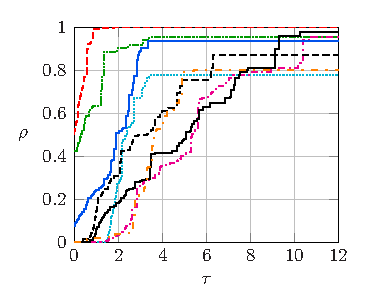
\includegraphics{lexample_fig1}
%  \caption{Example figure using external image files.}
%  \label{fig:testfig}
%\end{figure}
%
%\Cref{tab:foo} shows additional
%supporting evidence. 
%
%\begin{table}[htbp]
%\footnotesize
%\caption{Example table.}\label{tab:foo}
%\begin{center}
%  \begin{tabular}{|c|c|c|} \hline
%   Species & \bf Mean & \bf Std.~Dev. \\ \hline
%    1 & 3.4 & 1.2 \\
%    2 & 5.4 & 0.6 \\ 
%    3 & 7.4 & 2.4 \\ 
%    4 & 9.4 & 1.8 \\ \hline
%  \end{tabular}
%\end{center}
%\end{table}
%
%\lipsum[51]
%
%\section{Discussion of \texorpdfstring{{\boldmath$Z=X \cup Y$}}{Z = X union Y}}
%
%\lipsum[76]
%
%\section{Conclusions}
%\label{sec:conclusions}
%
%Some conclusions here.
%
%
%\appendix
%\section{An example appendix} 
%\lipsum[71]
%
%\begin{lemma}
%Test Lemma.
%\end{lemma}


\section*{Acknowledgments}
We would like to acknowledge the assistance of volunteers in putting
together this example manuscript and supplement.

\bibliographystyle{siamplain}
\bibliography{references}
\end{document}
